\documentclass{ximera}

%\usepackage{todonotes}

\newcommand{\todo}{}

\usepackage{tkz-euclide}
\tikzset{>=stealth} %% cool arrow head
\tikzset{shorten <>/.style={ shorten >=#1, shorten <=#1 } } %% allows shorter vectors

\usepackage{tkz-tab}  %% sign charts
\usetikzlibrary{decorations.pathreplacing} 

\usetikzlibrary{backgrounds} %% for boxes around graphs
\usetikzlibrary{shapes,positioning}  %% Clouds and stars
\usetikzlibrary{matrix} %% for matrix
\usepgfplotslibrary{polar} %% for polar plots
\usetkzobj{all}
\usepackage[makeroom]{cancel} %% for strike outs
%\usepackage{mathtools} %% for pretty underbrace % Breaks Ximera
\usepackage{multicol}

\usepackage{polynom}



\usepackage[many]{tcolorbox}  %% for titled boxes
\newtcolorbox{xbox}[1]{%
    tikznode boxed title,
    enhanced,
    arc=0mm,
    interior style={white},
    attach boxed title to top center= {yshift=-\tcboxedtitleheight/2},
    fonttitle=\bfseries,
    colbacktitle=white,coltitle=black,
    boxed title style={size=normal,colframe=white,boxrule=0pt},
    title={#1}}


\usepackage{array}
\setlength{\extrarowheight}{+.1cm}   
\newdimen\digitwidth
\settowidth\digitwidth{9}
\def\divrule#1#2{
\noalign{\moveright#1\digitwidth
\vbox{\hrule width#2\digitwidth}}}





\newcommand{\RR}{\mathbb R}
\newcommand{\R}{\mathbb R}
\newcommand{\N}{\mathbb N}
\newcommand{\Z}{\mathbb Z}

%\renewcommand{\d}{\,d\!}
\renewcommand{\d}{\mathop{}\!d}
\newcommand{\dd}[2][]{\frac{\d #1}{\d #2}}
\newcommand{\pp}[2][]{\frac{\partial #1}{\partial #2}}
\renewcommand{\l}{\ell}
\newcommand{\ddx}{\frac{d}{\d x}}
\newcommand{\ddt}{\frac{d}{\d t}}

\newcommand{\zeroOverZero}{\ensuremath{\boldsymbol{\tfrac{0}{0}}}}
\newcommand{\inftyOverInfty}{\ensuremath{\boldsymbol{\tfrac{\infty}{\infty}}}}
\newcommand{\zeroOverInfty}{\ensuremath{\boldsymbol{\tfrac{0}{\infty}}}}
\newcommand{\zeroTimesInfty}{\ensuremath{\small\boldsymbol{0\cdot \infty}}}
\newcommand{\inftyMinusInfty}{\ensuremath{\small\boldsymbol{\infty - \infty}}}
\newcommand{\oneToInfty}{\ensuremath{\boldsymbol{1^\infty}}}
\newcommand{\zeroToZero}{\ensuremath{\boldsymbol{0^0}}}
\newcommand{\inftyToZero}{\ensuremath{\boldsymbol{\infty^0}}}



\newcommand{\numOverZero}{\ensuremath{\boldsymbol{\tfrac{\#}{0}}}}
\newcommand{\dfn}{\textbf}
%\newcommand{\unit}{\,\mathrm}
\newcommand{\unit}{\mathop{}\!\mathrm}
\newcommand{\eval}[1]{\bigg[ #1 \bigg]}
\newcommand{\seq}[1]{\left( #1 \right)}
\renewcommand{\epsilon}{\varepsilon}
\renewcommand{\iff}{\Leftrightarrow}

\DeclareMathOperator{\arccot}{arccot}
\DeclareMathOperator{\arcsec}{arcsec}
\DeclareMathOperator{\arccsc}{arccsc}
\DeclareMathOperator{\si}{Si}
\DeclareMathOperator{\proj}{proj}
\DeclareMathOperator{\scal}{scal}


\newcommand{\tightoverset}[2]{% for arrow vec
  \mathop{#2}\limits^{\vbox to -.5ex{\kern-0.75ex\hbox{$#1$}\vss}}}
\newcommand{\arrowvec}[1]{\tightoverset{\scriptstyle\rightharpoonup}{#1}}
\renewcommand{\vec}{\mathbf}
\newcommand{\veci}{\vec{i}}
\newcommand{\vecj}{\vec{j}}
\newcommand{\veck}{\vec{k}}
\newcommand{\vecl}{\boldsymbol{\l}}

\newcommand{\dotp}{\bullet}
\newcommand{\cross}{\boldsymbol\times}
\newcommand{\grad}{\boldsymbol\nabla}
\newcommand{\divergence}{\grad\dotp}
\newcommand{\curl}{\grad\cross}
%\DeclareMathOperator{\divergence}{divergence}
%\DeclareMathOperator{\curl}[1]{\grad\cross #1}


\colorlet{textColor}{black} 
\colorlet{background}{white}
\colorlet{penColor}{blue!50!black} % Color of a curve in a plot
\colorlet{penColor2}{red!50!black}% Color of a curve in a plot
\colorlet{penColor3}{red!50!blue} % Color of a curve in a plot
\colorlet{penColor4}{green!50!black} % Color of a curve in a plot
\colorlet{penColor5}{orange!80!black} % Color of a curve in a plot
\colorlet{fill1}{penColor!20} % Color of fill in a plot
\colorlet{fill2}{penColor2!20} % Color of fill in a plot
\colorlet{fillp}{fill1} % Color of positive area
\colorlet{filln}{penColor2!20} % Color of negative area
\colorlet{fill3}{penColor3!20} % Fill
\colorlet{fill4}{penColor4!20} % Fill
\colorlet{fill5}{penColor5!20} % Fill
\colorlet{gridColor}{gray!50} % Color of grid in a plot

\newcommand{\surfaceColor}{violet}
\newcommand{\surfaceColorTwo}{redyellow}
\newcommand{\sliceColor}{greenyellow}




\pgfmathdeclarefunction{gauss}{2}{% gives gaussian
  \pgfmathparse{1/(#2*sqrt(2*pi))*exp(-((x-#1)^2)/(2*#2^2))}%
}


%%%%%%%%%%%%%
%% Vectors
%%%%%%%%%%%%%

%% Simple horiz vectors
\renewcommand{\vector}[1]{\left\langle #1\right\rangle}


%% %% Complex Horiz Vectors with angle brackets
%% \makeatletter
%% \renewcommand{\vector}[2][ , ]{\left\langle%
%%   \def\nextitem{\def\nextitem{#1}}%
%%   \@for \el:=#2\do{\nextitem\el}\right\rangle%
%% }
%% \makeatother

%% %% Vertical Vectors
%% \def\vector#1{\begin{bmatrix}\vecListA#1,,\end{bmatrix}}
%% \def\vecListA#1,{\if,#1,\else #1\cr \expandafter \vecListA \fi}

%%%%%%%%%%%%%
%% End of vectors
%%%%%%%%%%%%%

%\newcommand{\fullwidth}{}
%\newcommand{\normalwidth}{}



%% makes a snazzy t-chart for evaluating functions
%\newenvironment{tchart}{\rowcolors{2}{}{background!90!textColor}\array}{\endarray}

%%This is to help with formatting on future title pages.
\newenvironment{sectionOutcomes}{}{} 



%% Flowchart stuff
%\tikzstyle{startstop} = [rectangle, rounded corners, minimum width=3cm, minimum height=1cm,text centered, draw=black]
%\tikzstyle{question} = [rectangle, minimum width=3cm, minimum height=1cm, text centered, draw=black]
%\tikzstyle{decision} = [trapezium, trapezium left angle=70, trapezium right angle=110, minimum width=3cm, minimum height=1cm, text centered, draw=black]
%\tikzstyle{question} = [rectangle, rounded corners, minimum width=3cm, minimum height=1cm,text centered, draw=black]
%\tikzstyle{process} = [rectangle, minimum width=3cm, minimum height=1cm, text centered, draw=black]
%\tikzstyle{decision} = [trapezium, trapezium left angle=70, trapezium right angle=110, minimum width=3cm, minimum height=1cm, text centered, draw=black]


\outcome{Use the first derivative to determine whether a function is increasing or decreasing.}
\outcome{Identify the relationships between the function and its first and second derivatives.}
\outcome{Sketch a graph of the second derivative, given the original function.}
\outcome{Sketch a graph of the original function, given the graph of its first and second derivatives.}
\outcome{State the relationship between concavity and the second derivative.}

\title[Dig-In:]{Concavity}

\begin{document}
\begin{abstract}
  Here we examine what the second derivative tells us about the
  geometry of functions.
\end{abstract}
\maketitle


So far, we know how to determine if a function is increasing or decreasing by looking at the sign of its
derivative.  If all we know about $f$ is the increasing/decreasing information, we no not have enough
information to say how $f$ is behaving accurately enough.  Consider the following four possibilities:

\begin{image}
  \begin{tikzpicture}
    \draw (0,0) -- (0,12);
    \draw (0,0) -- (12,0);
    \draw (6,0) -- (6,12);
    \draw (0,6) -- (12,6);
    \draw (12,0) -- (12,12);
    \draw (0,12) -- (12,12);
    
    \node at (3,12.4) {\Large $f$ decreasing};
    \node at (9,12.4) {\Large$f$ increasing};
    
    \draw [penColor,ultra thick,domain=180:270] plot ({2*cos(\x)+4}, {2*sin(\x)+11});
    \draw [penColor,ultra thick,domain=270:360] plot ({2*cos(\x)+8}, {2*sin(\x)+11});
    \draw [penColor,ultra thick,domain=0:90] plot ({2*cos(\x)+2}, {2*sin(\x)+3});
    \draw [penColor,ultra thick,domain=180:90] plot ({2*cos(\x)+10}, {2*sin(\x)+3});

  \end{tikzpicture}
\end{image}

In both graphs in the left-hand column, $f$ is decreasing.  In both graphs in the right-hand column,
$f$ is increasing.  What is the difference between the two rows?  Their concavity.
\begin{definition}\index{concave up}\index{concave down}
	Let $f$ be a  function differentiable on an open interval $I$.\\
		We say that the graph of  $f$ is \textbf{concave up} on $I$ if  $f'$, the derivative of $f$, is \textbf{increasing} on $I$.\\
		We say that the graph of  $f$ is \textbf{concave down} on $I$ if $f'$, the derivative of $f$, is \textbf{decreasing} on $I$.
\end{definition}
That is, the graph of $f$ is concave up if the graph locally lies above its tangent lines, and is concave down if the graph locally lies below its tangent lines.

The graphs of two functions, $f$ and $g$, both increasing on the given interval, are given below.
\begin{image}
  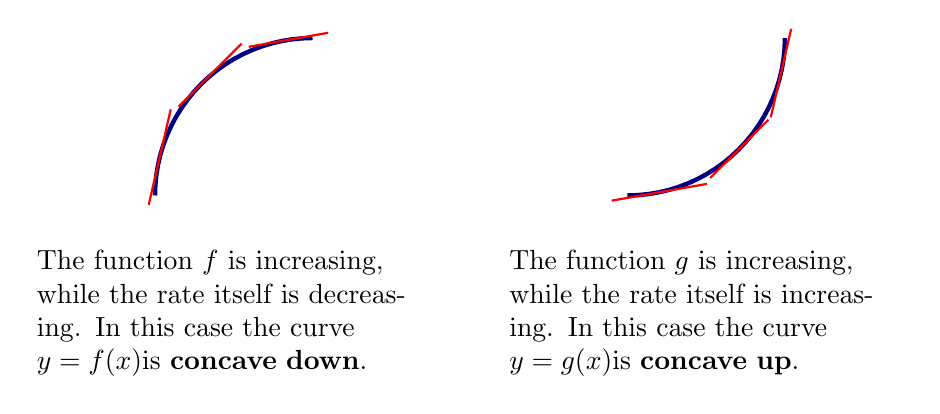
\begin{tikzpicture}
    \draw [penColor,  ultra thick,domain=180:270] plot ({2*cos(\x)+4},{9-2*sin(\x)});
    \draw [penColor, ultra thick,domain=270:360] plot ({2*cos(\x)+8}, {2*sin(\x)+11});
    \draw [color=red,thick, domain=1.92:2.2] plot({\x},{cot(193)*(\x-(2*cos(193)+4))+9-2*sin(193)});
    \draw [color=red, thick, domain=2.3:3.1] plot({\x},{cot(225)*(\x-(2*cos(225)+4))+9-2*sin(225)});    
    \draw [color=red, thick, domain=3.19:4.2] plot({\x},{cot(260)*(\x-(2*cos(260)+4))+9-2*sin(260)});
    \draw [color=red, thick, domain=7.8:9.01] plot({\x},{-cot(280)*(\x-(2*cos(280)+8))+11+2*sin(280)});
    \draw [color=red, thick, domain=9.05:9.79] plot({\x},{-cot(315)*(\x-(2*cos(315)+8))+11+2*sin(315)});
    \draw [color=red, thick, domain=9.82:10.08] plot({\x},{-cot(347)*(\x-(2*cos(347)+8))+11+2*sin(347)});
    \node at (3,7.5) [text width=5cm] {
      The function $f$ is increasing, while the rate itself is decreasing.
      In this case the curve  $y=f(x)$is \dfn{concave down}.};
    \node at (9,7.5) [text width=5cm] {
      The function $g$ is increasing, while the rate itself is increasing.
      In this case the curve  $y=g(x)$is \dfn{concave up}.};
  \end{tikzpicture}
\end{image}

\begin{example}
A graph of $y=f(x)$ is given below, with domain $\left(-\frac{3}{2} , \frac{3}{2} \right)$.
        \begin{image}
    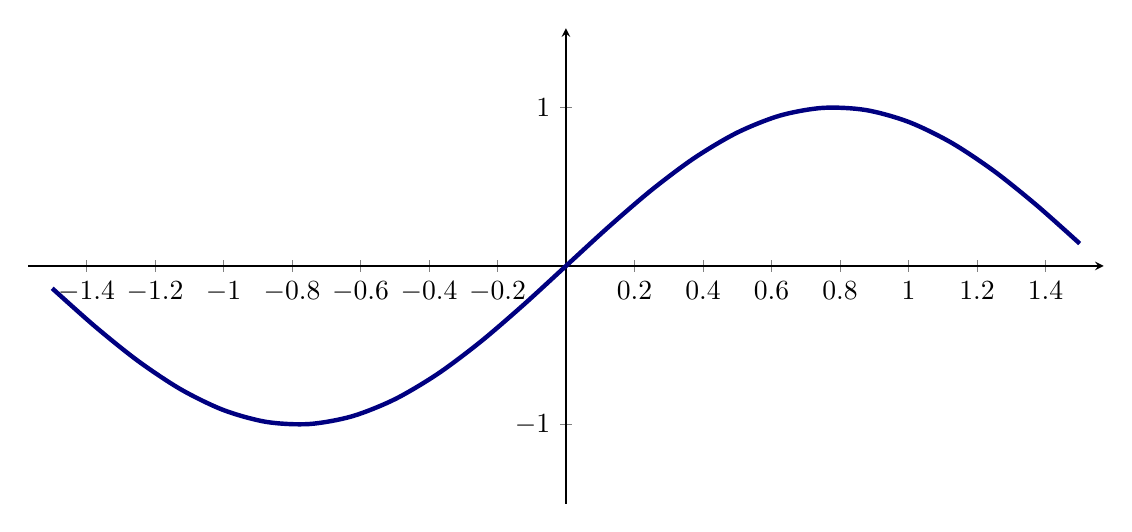
\begin{tikzpicture}
    \begin{axis}[
        xmin=-1.57,xmax=1.57,ymin=-1.5,ymax=1.5,
        axis lines=center,
        width=6in,
        height=3in,
        every axis y label/.style={at=(current axis.above origin),anchor=south},
        every axis x label/.style={at=(current axis.right of origin),anchor=west},
      ]
      \addplot [penColor,ultra thick,domain=-1.5:1.5,smooth] {sin(2*deg(x))};

    \end{axis}
  \end{tikzpicture}
  \end{image}
On what intervals is $f$ concave up?  On what intervals is $f$ concave down?
\begin{explanation}
	Let's draw some tangent lines on the graph.
	        \begin{image}
    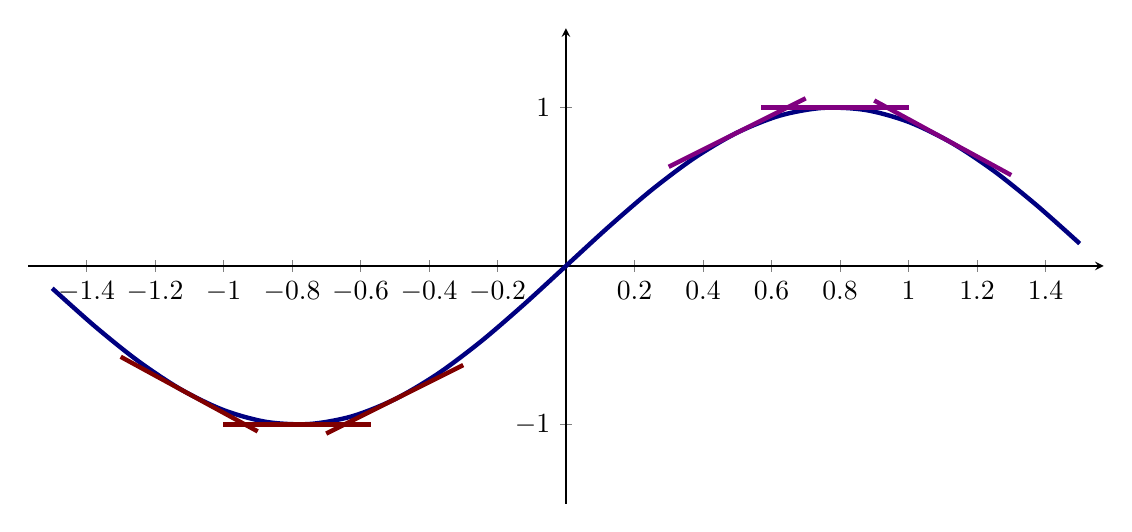
\begin{tikzpicture}
    \begin{axis}[
        xmin=-1.57,xmax=1.57,ymin=-1.5,ymax=1.5,
        axis lines=center,
        width=6in,
        height=3in,
        every axis y label/.style={at=(current axis.above origin),anchor=south},
        every axis x label/.style={at=(current axis.right of origin),anchor=west},
      ]
      \addplot [penColor,ultra thick,domain=-1.5:1.5,smooth] {sin(2*deg(x))};
      \addplot [penColor2,ultra thick,domain=-1:-0.57,smooth] {-1};
      \addplot [penColor2,ultra thick,domain=-0.7:-0.3,smooth] {2*cos(2*deg(-0.5))*(x+0.5)+sin(2*deg(-0.5))};
      \addplot [penColor2,ultra thick,domain=-1.3:-0.9,smooth] {2*cos(2*deg(-1.1))*(x+1.1)+sin(2*deg(-1.1))};
      \addplot [penColor3,ultra thick,domain=0.9:1.3,smooth] {2*cos(2*deg(1.1))*(x-1.1)+sin(2*deg(1.1))};
      \addplot [penColor3,ultra thick,domain=0.3:0.7,smooth] {2*cos(2*deg(0.5))*(x-0.5)+sin(2*deg(0.5))};
      \addplot [penColor3,ultra thick,domain=0.57:1,smooth] {1};
    \end{axis}
  \end{tikzpicture}
  \end{image}
  
  The graph is above the tangent lines for $x$ in $\left(-\frac{3}{2}, 0\right)$, and below the tangent lines we sketched on $\left(0, \frac{3}{2}\right)$.
  
  Therefore, $f$ is concave up on $\left(\answer{-\frac{3}{2}}, \answer{0}\right)$, and concave down on $\left(\answer{0}, \answer{\frac{3}{2}}\right)$.
\end{explanation}
\end{example}
In that example, examine the intervals where $f$ was concave up.  At the beginning of that interval, $f$ was decreasing, and at the end, $f$ was increasing.
The slopes in that interval increased from a negative value to a positive value.  In the interval where $f$ was concave down, the slopes started positive
and ended negative.  The slopes in that interval were decreasing.

We know that the sign of the derivative tells us whether a function is increasing or decreasing at some point. Likewise, the sign of the
second derivative $f''(x)$ tells us whether $f'(x)$ is increasing or decreasing at $x$.  Let's use this to add more details into the chart from above.

\begin{image}
  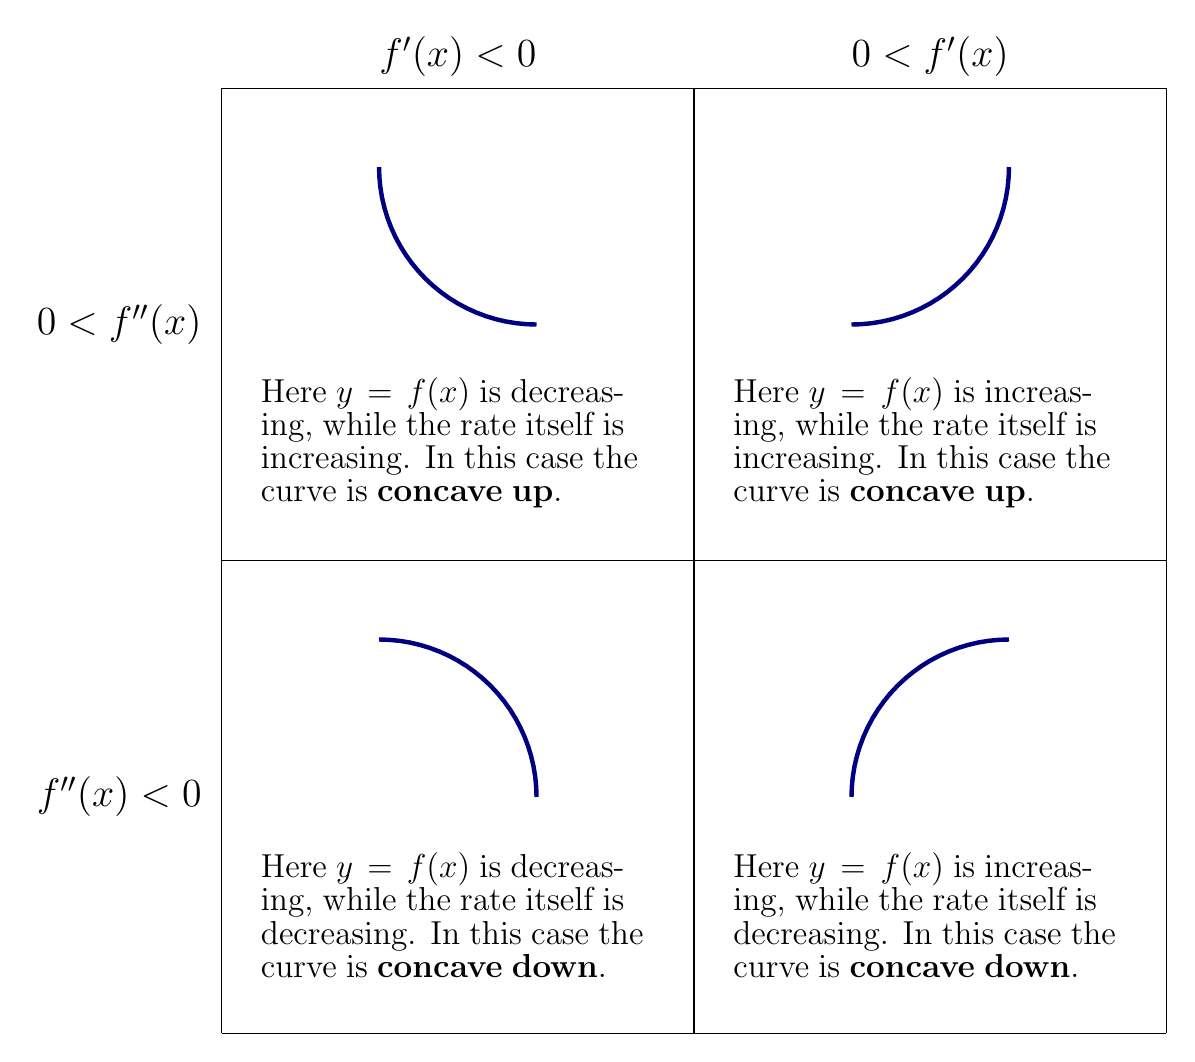
\begin{tikzpicture}
    \draw (0,0) -- (0,12);
    \draw (0,0) -- (12,0);
    \draw (6,0) -- (6,12);
    \draw (0,6) -- (12,6);
    \draw (12,0) -- (12,12);
    \draw (0,12) -- (12,12);
    
    \node at (-1.3,9) {\Large$0<f''(x)$};
    \node at (-1.3,3) {\Large$f''(x)<0$};
    \node at (3,12.4) {\Large$f'(x)<0$};
    \node at (9,12.4) {\Large$0<f'(x)$};
    
    \draw [penColor,ultra thick,domain=180:270] plot ({2*cos(\x)+4}, {2*sin(\x)+11});
    \draw [penColor,ultra thick,domain=270:360] plot ({2*cos(\x)+8}, {2*sin(\x)+11});
    \draw [penColor,ultra thick,domain=0:90] plot ({2*cos(\x)+2}, {2*sin(\x)+3});
    \draw [penColor,ultra thick,domain=180:90] plot ({2*cos(\x)+10}, {2*sin(\x)+3});

    \node at (3,7.5) [text width=5cm] {\large
      Here $y=f(x)$ is decreasing, while the rate itself is increasing.
      In this case the curve is \dfn{concave up}.};

    \node at (9,7.5) [text width=5cm] {\large
      Here $y=f(x)$ is increasing, while the rate itself is increasing.
      In this case the curve is \dfn{concave up}.};

    \node at (3,1.5) [text width=5cm] {\large
      Here $y=f(x)$ is decreasing, while the rate itself is decreasing.
      In this case the curve is \dfn{concave down}.};

    \node at (9,1.5) [text width=5cm] {\large
      Here $y=f(x)$ is increasing, while the rate itself is decreasing.
      In this case the curve is \dfn{concave down}.};
  \end{tikzpicture}
\end{image}

If we are trying to understand the shape of the graph of a function,
knowing where it is concave up and concave down helps us to get a more
accurate picture. It is worth summarizing what we have seen already in
to a single theorem.

\begin{theorem}[Test for Concavity]\index{concavity test} 
	Let $I$ be an open interval.
	\begin{enumerate}
		\item If $f''(x)>0$ for all $x$ in $I$, then the graph of $f$ is  concave up on $I$.
		\item If $f''(x)<0$ for all $x$ in $I$, then the graph of $f$ is  concave down on $I$.
	\end{enumerate}
\end{theorem}


\begin{example}
  Let $f$ be a continuous function and suppose that:
  \begin{itemize}
  \item $f'(x) > 0$ for $-1< x<1$.
  \item $f'(x) < 0$ for $-2< x<-1$ and $1<x<2$.
  \item $f''(x) > 0$ for $-2<x<0$ and $1<x< 2$.
  \item $f''(x) < 0$ for $0<x< 1$.  
  \end{itemize}
  Sketch a possible graph of $f$.
  \begin{explanation}
    Start by marking where the derivative changes sign and indicate
    intervals where $f$ is increasing and intervals $f$ is
    decreasing. The function $f$ has a negative derivative from $-2$
    to $x=\answer[given]{-1}$. This means that $f$ is
    \wordChoice{\choice{increasing}\choice[correct]{decreasing}} on
    this interval. The function $f$ has a positive derivative from
    $x=\answer[given]{-1}$ to $x=\answer[given]{1}$. This means that
    $f$ is
    \wordChoice{\choice[correct]{increasing}\choice{decreasing}} on
    this interval. Finally, The function $f$ has a negative derivative
    from $x=\answer[given]{1}$ to $2$. This means that $f$ is
    \wordChoice{\choice{increasing}\choice[correct]{decreasing}} on
    this interval.
  \begin{image}
    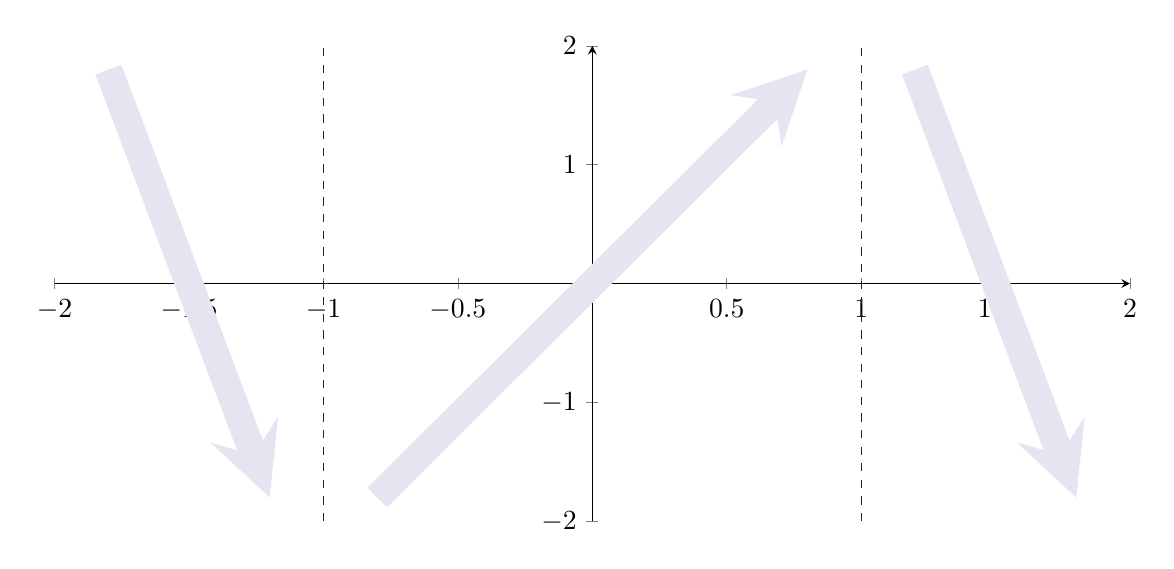
\begin{tikzpicture}
    \begin{axis}[
        xmin=-2,xmax=2,ymin=-2,ymax=2,
        axis lines=center,
        width=6in,
        height=3in,
        every axis y label/.style={at=(current axis.above origin),anchor=south},
        every axis x label/.style={at=(current axis.right of origin),anchor=west},
      ]
      \addplot [dashed, penColor2] plot coordinates {(-1,-2) (-1,2)}; %% Critical points
      \addplot [dashed, penColor2] plot coordinates {(1,-2) (1,2)}; %% Critical points

      \addplot [->, line width=10, penColor!10!background] plot coordinates {(-1+.2,-2+.2) (1-.2,2-.2)};
      \addplot [->, line width=10, penColor!10!background] plot coordinates {(-2+.2,2-.2) (-1-.2,-2+.2)};
      \addplot [->, line width=10, penColor!10!background] plot coordinates {(1+.2,2-.2) (2-.2,-2+.2)}; 
      
      %\addplot [very thick,penColor,smooth, domain=(-2:2)] {x^3+x^2-2*x)};
    \end{axis}
  \end{tikzpicture}
  \end{image}
  Now we should sketch the concavity: \wordChoice{\choice[correct]{concave up}\choice{concave down}} when the second
  derivative is positive, \wordChoice{\choice{concave up}\choice[correct]{concave down}} when the second derivative is
  negative.
    \begin{image}
    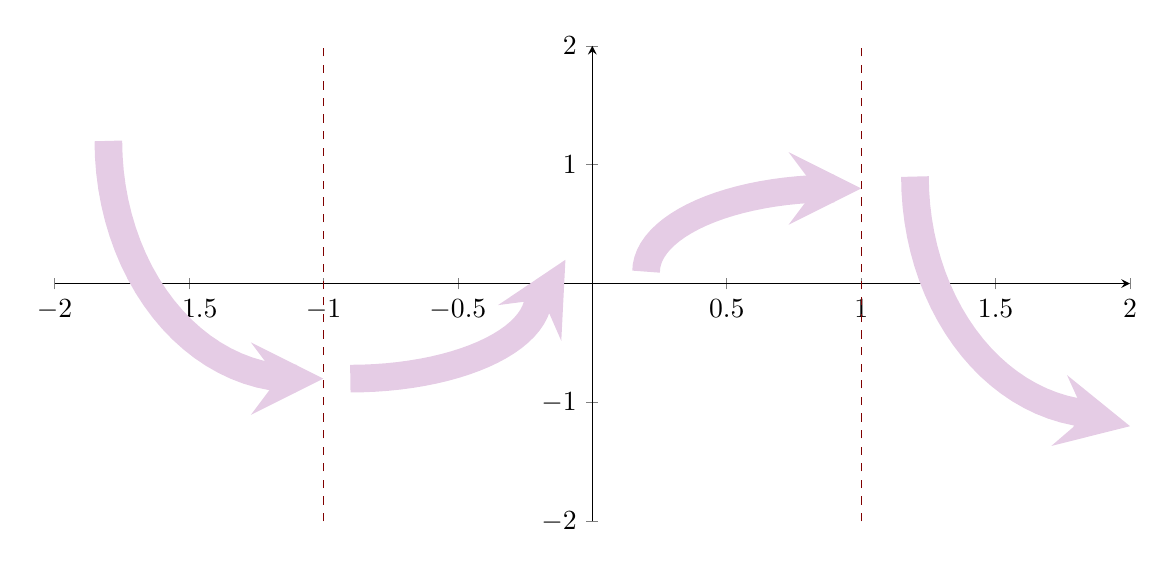
\begin{tikzpicture}
    \begin{axis}[
        xmin=-2,xmax=2,ymin=-2,ymax=2,
        axis lines=center,
        width=6in,
        height=3in,
        every axis y label/.style={at=(current axis.above origin),anchor=south},
        every axis x label/.style={at=(current axis.right of origin),anchor=west},
      ]
      \addplot [dashed, penColor2] plot coordinates {(-1,-2) (-1,2)}; %% Critical points
      \addplot [dashed, penColor2] plot coordinates {(1,-2) (1,2)}; %% Critical points

      %\addplot [->, line width=10, penColor!10!background] plot coordinates {(-1+.2,-2+.2) (1-.2,2-.2)};
      %\addplot [->, line width=10, penColor!10!background] plot coordinates {(-2+.2,2-.2) (-1-.2,-2+.2)};
      %\addplot [->, line width=10, penColor!10!background] plot coordinates {(1+.2,2-.2) (2-.2,-2+.2)};

      \addplot [penColor3!20!background,line width=10,domain=180:270] ({-1.1+.7*cos(x)}, {1.2+2*sin(x)});
      \addplot [penColor3!20!background,line width=10,domain=270:360] ({-.9+.7*cos(x)}, {-.1+.7*sin(x)});
      \addplot [penColor3!20!background,line width=10,domain=180:90] ({.9+.7*cos(x)}, {.1+.7*sin(x)});
      \addplot [penColor3!20!background,line width=10,domain=180:265] ({1.9+.7*cos(x)}, {.9+ 2*sin(x)});

      \addplot [->, line width=10, penColor3!20!background] plot coordinates {(-1.1,-.1-.7) (-1,-.1-.7)};
      \addplot [->, line width=10, penColor3!20!background] plot coordinates {(.9,.1+.7) (1,.1+.7)};
      
      \addplot [->, line width=10, penColor3!20!background] plot coordinates {(-.9+.7,-.2) (-.9+.8,.2)};
      \addplot [->, line width=10, penColor3!20!background] plot coordinates {(1.8,-1.1) (2,-1.2)};
      
      %\addplot [very thick,penColor,smooth, domain=(-2:2)] {x^3+x^2-2*x)};
    \end{axis}
  \end{tikzpicture}
    \end{image}
    Finally, we can sketch our curve:
        \begin{image}
    \begin{tikzpicture}
    \begin{axis}[
        xmin=-2,xmax=2,ymin=-2,ymax=2,
        axis lines=center,
        width=6in,
        height=3in,
        every axis y label/.style={at=(current axis.above origin),anchor=south},
        every axis x label/.style={at=(current axis.right of origin),anchor=west},
      ]
      \addplot [dashed, penColor2] plot coordinates {(-1,-2) (-1,2)}; %% Critical points
      \addplot [dashed, penColor2] plot coordinates {(1,-2) (1,2)}; %% Critical points

      \addplot [penColor,ultra thick,domain=-2:1,smooth] {(-x^3+3*x)*.5};
      \addplot [penColor,ultra thick,domain=1:2,smooth] {(-(x-3)^3+3*(x-3))*.5};
    \end{axis}
  \end{tikzpicture}
  \end{image}
  \end{explanation}
\end{example}

\end{document}
